\chapter{Исследовательская часть}
В данной части будет проведено исследование возможности выделения участков программы, которые могут быть использованы параллельно в алгоритме нахождения максимального элемента последовательности.

\section{Графовые модели для итеративного алгоритма}
Номера вершин графовых моделей соответствуют номерам строк кода, указанных в комментариях в листинге~\ref{list:iter}.

На рисунке~\ref{fig:risunok_4_1} продемонстрирована схема графа управления
\begin{figure}[H]
	\centering
	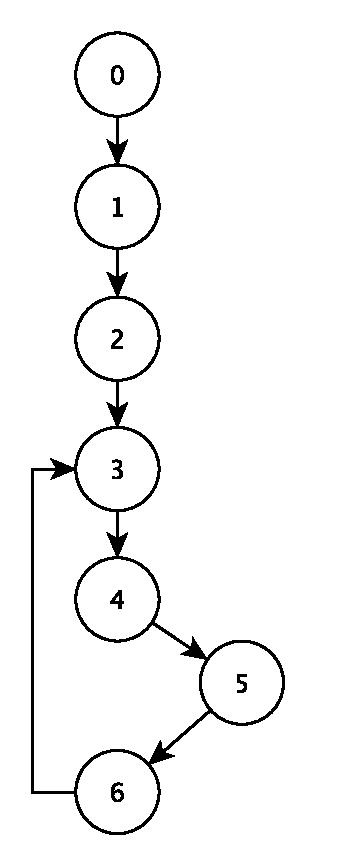
\includegraphics[width=0.35\textwidth]{images/AA4_1.pdf}
	\caption{Схема графа управления}
	\label{fig:risunok_4_1}
\end{figure}
На рисунке~\ref{fig:risunok_4_2} продемонстрирована схема информационного графа
\begin{figure}[H]
	\centering
	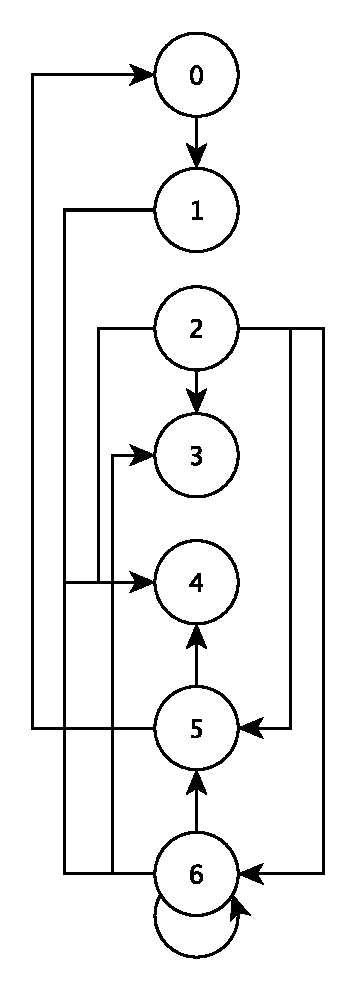
\includegraphics[width=0.35\textwidth]{images/AA4_2.pdf}
	\caption{Схема информационного графа}
	\label{fig:risunok_4_2}
\end{figure}

На рисунке~\ref{fig:risunok_4_3} продемонстрирована операционная история алгоритма нахождения максимального элемента последовательности из 5 элементов отсортированных в порядке возрастания.
\begin{figure}[H]
	\centering
	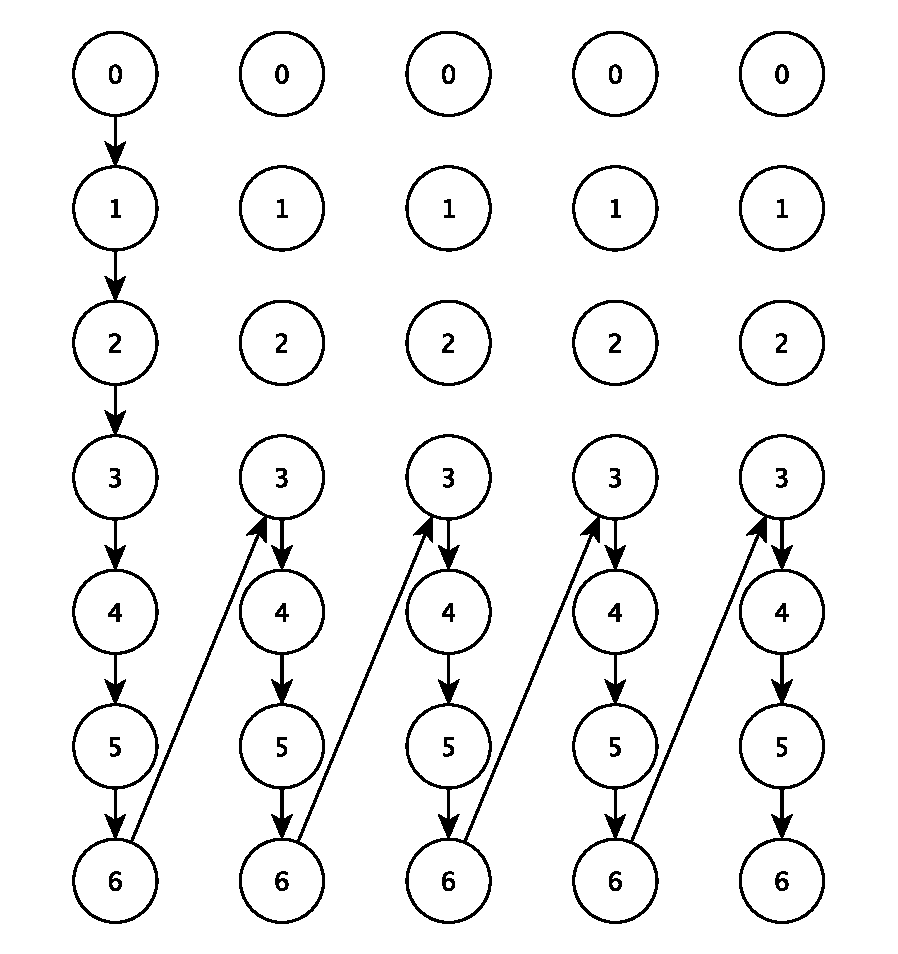
\includegraphics[width=0.85\textwidth]{images/AA4_3.pdf}
	\caption{Операционная история итеративного алгоритма}
	\label{fig:risunok_4_3}
\end{figure}

На рисунке~\ref{fig:risunok_4_4} продемонстрирована информационная история алгоритма нахождения максимального элемента последовательности из 5 элементов отсортированных в порядке возрастания.
\begin{figure}[H]
	\centering
	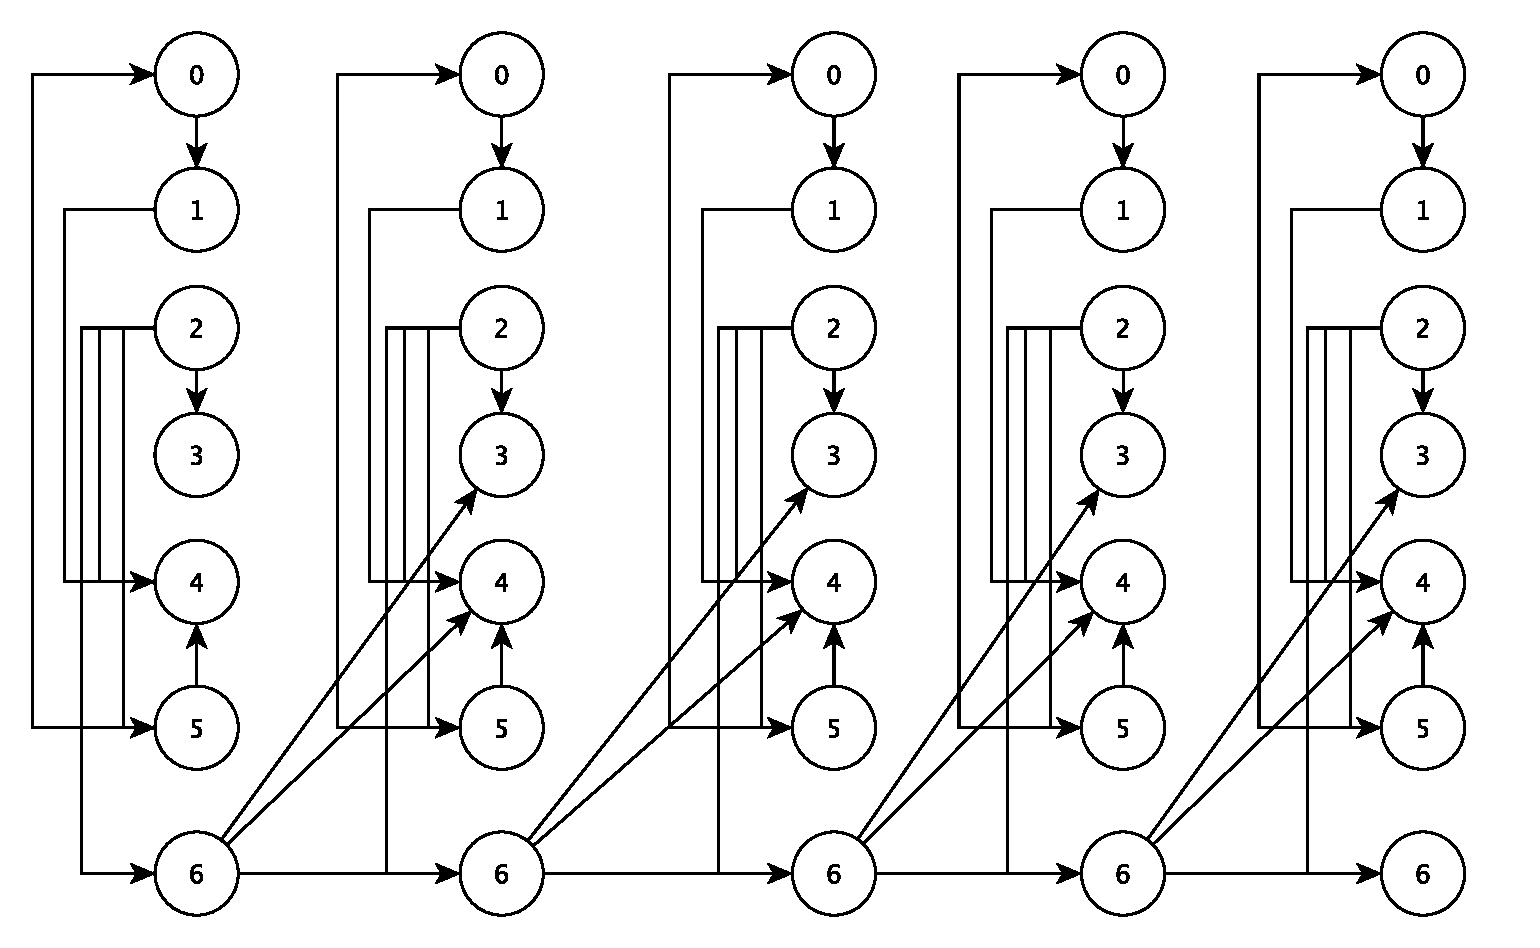
\includegraphics[width=1\textwidth]{images/AA4_4.pdf}
	\caption{Информационная история итеративного алгоритма}
	\label{fig:risunok_4_4}
\end{figure}

\section{Графовые модели для рекурсивного алгоритма}
Номера вершин графовых моделей соответствуют номерам строк кода, указанных в комментариях в листинге~\ref{list:rec}.

На рисунке~\ref{fig:risunok_4_5} продемонстрирована схема графа управления рекурсивного алгоритма.
\begin{figure}[H]
	\centering
	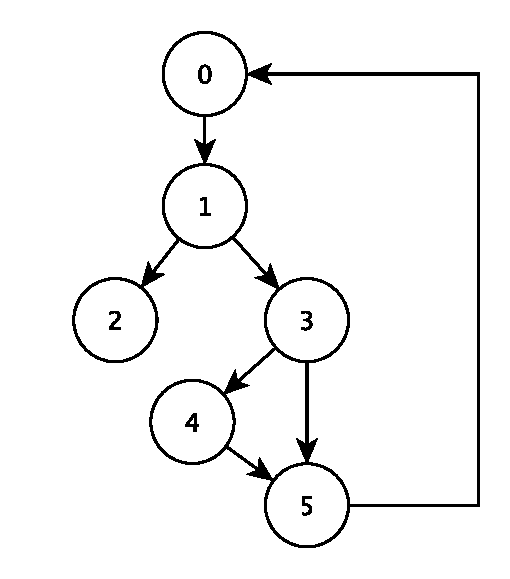
\includegraphics[width=0.45\textwidth]{images/AA4_5.pdf}
	\caption{Схема графа управления рекурсивного алгоритма}
	\label{fig:risunok_4_5}
\end{figure}
На рисунке~\ref{fig:risunok_4_6} продемонстрирована схема информационного графа рекурсивного алгоритма.рекурсивного алгоритма
\begin{figure}[H]
	\centering
	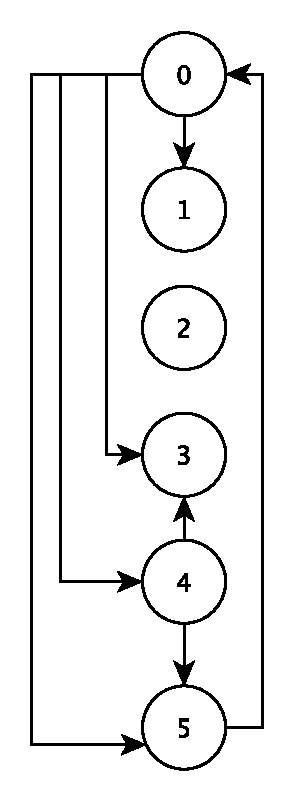
\includegraphics[width=0.3\textwidth]{images/AA4_6.pdf}
	\caption{Схема информационного графа рекурсивного алгоритма}
	\label{fig:risunok_4_6}
\end{figure}

На рисунке~\ref{fig:risunok_4_7} продемонстрирована операционная история рекурсивного алгоритма нахождения максимального элемента последовательности из 5 элементов отсортированных в порядке возрастания.
\begin{figure}[H]
	\centering
	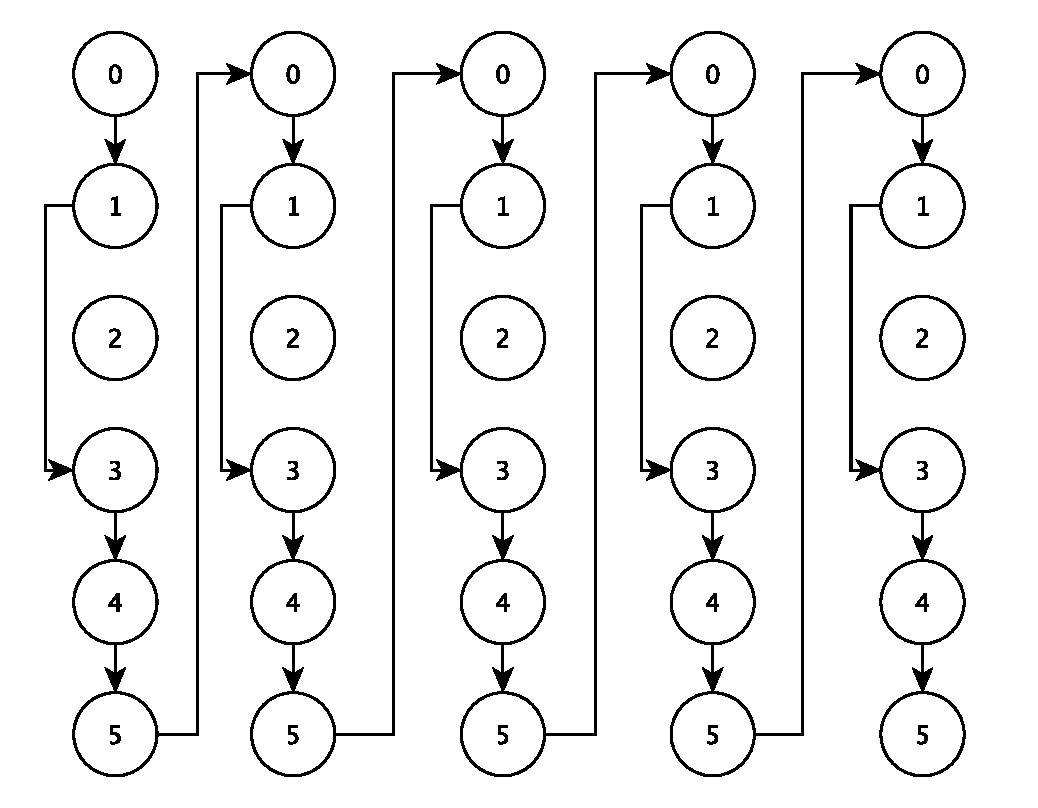
\includegraphics[width=0.85\textwidth]{images/AA4_7.pdf}
	\caption{Операционная история рекурсивного алгоритма}
	\label{fig:risunok_4_7}
\end{figure}

На рисунке~\ref{fig:risunok_4_8} продемонстрирована информационная история рекурсивного алгоритма нахождения максимального элемента последовательности из 5 элементов отсортированных в порядке возрастания.
\begin{figure}[H]
	\centering
	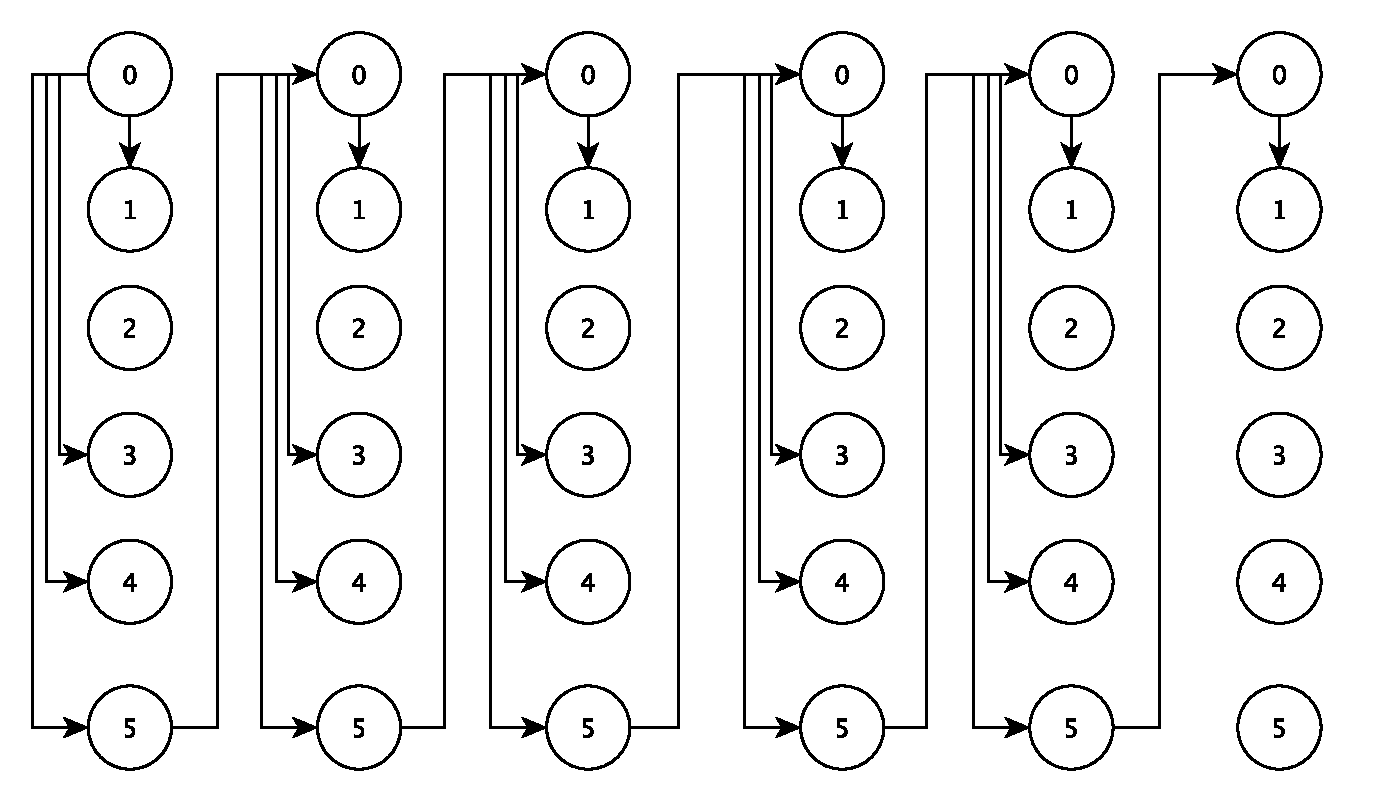
\includegraphics[width=1\textwidth]{images/AA4_8.pdf}
	\caption{Информационная история рекурсивного алгоритма}
	\label{fig:risunok_4_8}
\end{figure}

\section*{Вывод}
Никакие участки программы не могут выполняться параллельно, так как все операции зависят от предыдущих.

\clearpage
